%
%

%%-----------------------------------------------------
%%-----------------------------------------------------
\section{De rebajas}

%%-----------------------------------------------------
\begin{frame}
\frametitle{Markdown}

{\Large
\begin{itemize}
\item Primera version: 2004
\item Objetivo:
  \begin{quote}
  ``escribir usando un formato plano de texto, fácil de leer y fácil de escribir, que pueda ser convertido a HTML''
  \end{quote}
\item Uso creciente
\item Cada vez más herramientas
\item Cada vez más extensiones
\item README.md de GitHub
\end{itemize}
}

\begin{center}

\includegraphics[width=11cm]{figs/markdown-logo}
\end{center}

\end{frame}


%%-----------------------------------------------------
\begin{frame}[fragile]
\frametitle{Ejemplo (texto / HTML)}

\begin{columns}[T]
\begin{column}{.43\textwidth}

\begin{verbatim}
# Ejemplo

Esto es un pequeño ejemplo...

## Subtítulo

Ejemplos en los
[README.md de Git Hub]
(http://github.io "Git Hub")

Ejemplo de lista:
* Uno
* Dos
* Tres
\end{verbatim}

\end{column}%
\hfill%
\begin{column}{.53\textwidth}
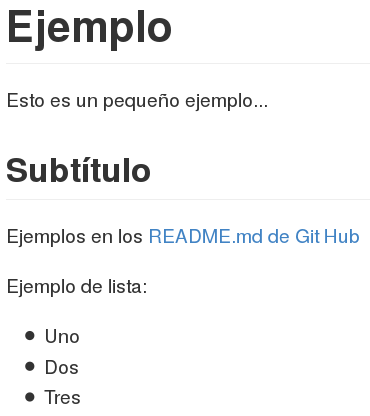
\includegraphics[width=6.5cm]{figs/markdown-ejemplo}
\end{column}%
\end{columns}

\end{frame}

%%-----------------------------------------------------
\begin{frame}
\frametitle{Marcado, herramientas}

Guías de marcado:
\begin{itemize}
\item Original \\
{\small \url{http://daringfireball.net/projects/markdown/syntax}} \\
\item GitHub \\
{\small \url{http://help.github.com/articles/github-flavored-markdown/}} \\
\item Pandoc \\
{\small \url{http://johnmacfarlane.net/pandoc/demo/example9/pandocs-markdown.html}} \\
\end{itemize}

Herramientas:
\begin{itemize}
\item Pandoc
\item Grip (Github Readme Instant Preview)
\item ...
\end{itemize}

\end{frame}

%%-----------------------------------------------------
\begin{frame}
\frametitle{Ejemplo: un libro con Markdown}

\begin{center}
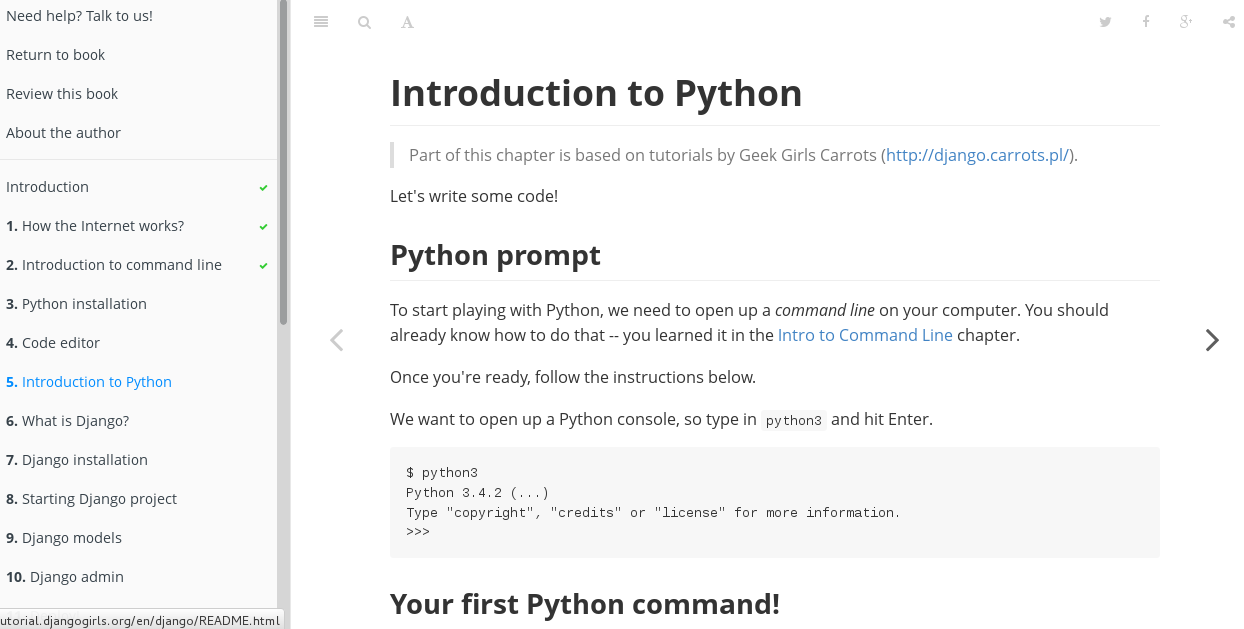
\includegraphics[width=11cm]{figs/markdown-book}
\end{center}

\begin{flushright}
\url{http://djangogirls.gitbooks.io/djangogirls-tutorial/} \\
\url{https://github.com/GitbookIO/gitbook} \\
\end{flushright}

\end{frame}
